\title{คาบเรียนที่ 2: มุมระหว่างเวกเตอร์ เวกเตอร์เชิงตั้งฉาก และผลคูณไขว้}
\frame{\titlepage}


\begin{frame}
\frametitle{สารบัญ}
\tableofcontents
\end{frame}

%%%%%%%%%%%%%
\section{มุมระหว่างเวกเตอร์}
\frame{\sectionpage}
%%%%%%%%%%%%%

\begin{frame}
\frametitle{มุมระหว่างเวกเตอร์}
\begin{defn}{}{}
กำหนดเวกเตอร์ $\vec{u}$ และ $\vec{v}$ โดยที่จุดเริ่มต้นอยู่ที่จุดกำเนิดเหมือนกัน แล้ว\alert{มุมระหว่างเวกเตอร์} $\theta$ คือมุมที่นับจากเวกเตอร์หนึ่งไปยังอีกเวกเตอร์หนึ่ง ซึ่ง $0 \leq \theta \leq \pi$
\end{defn}
\end{frame}

\begin{frame}
\begin{figure}[h!]
\centering
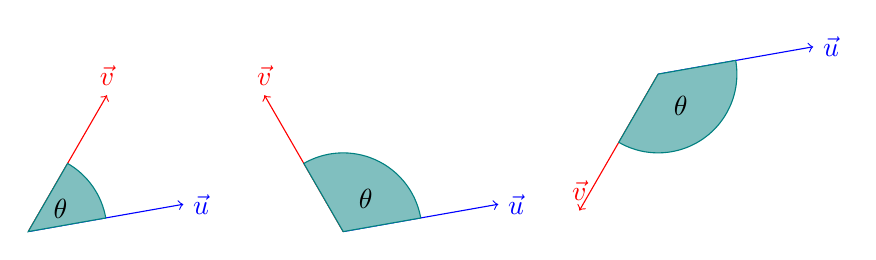
\begin{tikzpicture}
\draw[->, blue] (0,0) -- (10:2) node [right] {$\vec{u}$};
\draw[->, red] (0,0) -- (60:2) node [above] {$\vec{v}$};
\filldraw[fill = teal!50!white, draw = teal] (0,0) -- (10:1) arc [start angle = 10, end angle = 60, radius = 1] -- cycle;
\node at (35:0.5) {$\theta$};
\begin{scope}[xshift = 4cm]
\draw[->, blue] (0,0) -- (10:2) node [right] {$\vec{u}$};
\draw[->, red] (0,0) -- (120:2) node [above] {$\vec{v}$};
\filldraw[fill = teal!50!white, draw = teal] (0,0) -- (10:1) arc [start angle = 10, end angle = 120, radius = 1] -- cycle;
\node at (55:0.5) {$\theta$};
\end{scope}
\begin{scope}[xshift = 8cm, yshift = 2cm]
\draw[->, blue] (0,0) -- (10:2) node [right] {$\vec{u}$};
\draw[->, red] (0,0) -- (240:2) node [above] {$\vec{v}$};
\filldraw[fill = teal!50!white, draw = teal] (0,0) -- (240:1) arc [start angle = 240, end angle = 370, radius = 1] -- cycle;
\node at (305:0.5) {$\theta$};
\end{scope}
\end{tikzpicture}
\caption{มุม $\theta$ ระหว่างเวกเตอร์ $\vec{u}$ และ $\vec{v}$}
\end{figure}
\end{frame}

\begin{frame}
\begin{thm}{}{}
กำหนดให้ $\theta$ เป็นมุมระหว่าง $\vec{u}, \vec {v}$ แล้ว 
\begin{equation}
\cos \theta = \frac{\vec{u} \cdot \vec{v} }{\| \vec{u} \|\| \vec{v} \|}
\end{equation} \pa
นั่นคือ
\begin{equation}
\theta = \arccos \left( \frac{\vec{u} \cdot \vec{v} }{\| \vec{u} \|\| \vec{v} \|} \right), \quad 0 \leq \theta \leq \pi
\end{equation}
\end{thm}
\end{frame}

 
\begin{frame}[t]
\begin{ex}{}
จงหามุม $\theta$ ระหว่างเวกเตอร์  $\bv{1,4}$ และ $\bv{4,1}$
\end{ex}
\begin{sol} หาขนาดและผลคูณจุดดังนี้ \pa
\begin{eq*} 
\| \bv{1,4} \| \pa &=& \sqrt{1^2+4^2} = \sqrt{17} \pa \\
\| \bv{4,1} \| \pa &=& \sqrt{4^2+1^2} = \sqrt{17} \pa \\
\bv{1,4} \cdot \bv{4,1} \pa &=& (1\times 4) + (4 \times 1) = 8
\end{eq*}
ฉะนั้น \pa

\[\cos \theta = \frac{\vec{u} \cdot \vec{v} }{\| \vec{u} \|\| \vec{v} \|} \pa = \frac{8}{\sqrt{17}\times \sqrt{17}} \pa = \frac{8}{17}\]
นั่นคือ $\theta = \arccos \left( \frac{8}{17} \right)$
\end{sol}
\end{frame}

 
\begin{frame}[t]
\begin{ex}{}
จงหามุม $\theta$ ระหว่างเวกเตอร์  $\bv{-1,1,3}$ และ $\bv{0,3,-1}$
\end{ex}
\begin{sol} หาขนาดและผลคูณจุดดังนี้ \pa
\begin{eq*}
\| \bv{-1,1,3} \| \pa &=& \sqrt{(-1)^2+1^2+3^2} = \sqrt{11} \pa \\
\| \bv{0,3,-1} \| \pa &=& \sqrt{0^2+3^2+(-1)^2} = \sqrt{10} \pa \\
\bv{-1,1,3} \cdot \bv{0,3,-1} \pa &=& ((-1)\times 0) + (1 \times 3)  + (3 \times (-1))= 0
\end{eq*}
ฉะนั้น \pa
\[\cos \theta = \frac{\vec{u} \cdot \vec{v} }{\| \vec{u} \|\| \vec{v} \|} \pa = 0\]
นั่นคือ $\theta = \arccos 0 = \frac{\pi}{2}$
\end{sol}
\end{frame}

\begin{frame}[t]
เราทราบว่าเราสามารถใช้ผลคูณจุดหามุมระหว่างเวกเตอร์ได้ ทำให้เราสามารถสรุปกรณีต่าง ๆ ได้ดังต่อไปนี้
\begin{slide}
\begin{thm}{}{}
กำหนดเวกเตอร์ $\vec{u}$ และ $\vec{v}$ ที่ $\vec{u} \neq \vec{0}$ และ $\vec{v} \neq \vec{0}$ โดยที่ $\theta$ เป็นมุมระหว่างเวกเตอร์ทั้งสอง \pa
\begin{itemize}
\item ถ้า $\vec{u} \cdot \vec{v} = 0$ \pa แล้ว $\theta = \tfrac{\pi}{2}$ นั่นคือเวกเตอร์ทั้งสองตั้งฉากกัน เราใช้สัญลักษณ์ $\vec{u} \perp \vec{v}$ \pa
\item ถ้า $\vec{u} \cdot \vec{v} > 0$ \pa แล้ว $\theta$ เป็นมุมแหลม (นั่นคือ $0 \leq \theta < \tfrac{\pi}{2}$) \pa
\item ถ้า $\vec{u} \cdot \vec{v} < 0$ \pa แล้ว $\theta$ เป็นมุมป้าน (นั่นคือ $\tfrac{\pi}{2} < \theta \leq \pi$) \pa
\end{itemize}
\end{thm}
\end{slide}
\end{frame}

\begin{frame}
\begin{figure}[h!]
\centering
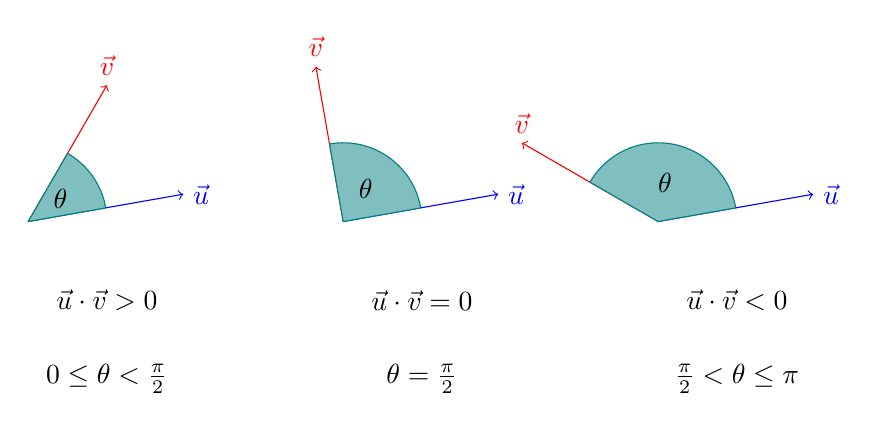
\begin{tikzpicture}
\draw[->, blue] (0,0) -- (10:2) node [right] {$\vec{u}$};
\draw[->, red] (0,0) -- (60:2) node [above] {$\vec{v}$};
\filldraw[fill = teal!50!white, draw = teal] (0,0) -- (10:1) arc [start angle = 10, end angle = 60, radius = 1] -- cycle; 
\node at (35:0.5) {$\theta$};
\node at (1,-1) {$\vec{u} \cdot \vec{v} > 0$};
\node at (1,-2) {$0 \leq \theta < \frac{\pi}{2}$};
\begin{scope}[xshift = 4cm]
\draw[->, blue] (0,0) -- (10:2) node [right] {$\vec{u}$};
\draw[->, red] (0,0) -- (100:2) node [above] {$\vec{v}$};
\filldraw[fill = teal!50!white, draw = teal] (0,0) -- (10:1) arc [start angle = 10, end angle = 100, radius = 1] -- cycle;
\node at (55:0.5) {$\theta$};
\node at (1,-1) {$\vec{u} \cdot \vec{v} = 0$};
\node at (1,-2) {$\theta = \frac{\pi}{2}$};
\end{scope}
\begin{scope}[xshift = 8cm]
\draw[->, blue] (0,0) -- (10:2) node [right] {$\vec{u}$};
\draw[->, red] (0,0) -- (150:2) node [above] {$\vec{v}$};
\filldraw[fill = teal!50!white, draw = teal] (0,0) -- (10:1) arc [start angle = 10, end angle = 150, radius = 1] -- cycle;
\node at (80:0.5) {$\theta$};
\node at (1,-1) {$\vec{u} \cdot \vec{v} < 0$};
\node at (1,-2) {$\frac{\pi}{2} < \theta \leq \pi$};
\end{scope}
\end{tikzpicture}
\caption{ความสัมพันธ์ระหว่างมุม $\theta$ และผลคูณจุด $\vec{u} \cdot \vec{v}$}
\end{figure}
\end{frame}

%%%%%%%%%%%%%
\section{โคไซน์แสดงทิศทาง}
\frame{\sectionpage}
%%%%%%%%%%%%%

\begin{frame}
\frametitle{โคไซน์แสดงทิศทาง}
\begin{slide}
ในปริภูมิสองมิติ เราสามารถกำหนดทิศทางของเวกเตอร์ $\vec{u} = \bv{u_1, u_2}$ ได้ด้วยการเทียบมุม $\theta$ กับแกน $x$ ซึ่งหาได้จาก
\[\tan \theta = \frac{u_1}{u_2}\]

\begin{figure}[h!]
\centering
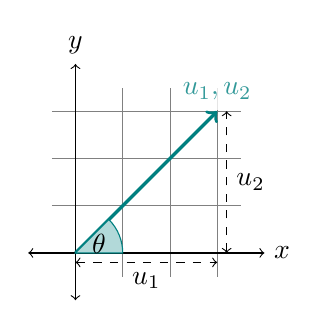
\begin{tikzpicture}[scale = 0.6]
\draw[help lines] (-0.5,-0.5) grid (3.5,3.5);
\draw[<->] (-1,0) -- (4,0) node [pos=1, right] {$x$};
\draw[<->] (0,-1) -- (0,4) node [pos=1, above] {$y$};
\draw[->, very thick, teal] (0,0) -- (3,3) node [fill = white, fill opacity = 0.8, pos=1, above] {$\bv{\red{u_1},\blue{u_2}}$};
\draw[<->, dashed] (0,-0.2) -- (3,-0.2) node [pos = 0.5, below] {$\red{u_1}$};
\draw[<->, dashed] (3.2,0) -- (3.2,3) node [pos = 0.5, right] {$\blue{u_2}$};
\filldraw[fill = teal!30!white, draw = teal] (0,0) -- (1,0) arc [start angle = 0, end angle = 45, radius = 1] -- cycle;
\node at (0.5,0.2) {$\theta$};
\end{tikzpicture}
\caption{มุม $\theta$ แสดงทิศทางของเวกเตอร์ $\vec{u}$}
\end{figure}
\end{slide}
\end{frame}

\begin{frame}
แต่ในปริภูมิสามมิติ เราจำเป็นต้องระบุว่าเราหามุมเทียบกับแกนใด เราจึงต้องนิยามมุมแสดงทิศทางดังนี้

\begin{figure}[h!]
\centering
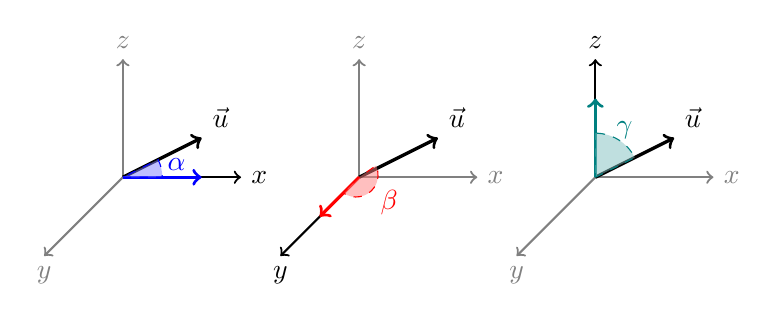
\begin{tikzpicture}
\draw[->, thick] (0,0) -- (1.5,0) node[right] {$x$};
\draw[->, thick, gray] (0,0) -- (-1,-1) node[left, below] {$y$};
\draw[->, thick, gray] (0,0) -- (0,1.5) node[above] {$z$};
\draw[->, very thick] (0,0) -- (1,0.5) node [above right] {$\vec{u}$};
\draw[->, blue, very thick] (0,0) -- (1,0);
\filldraw[fill = blue!50!white, fill opacity = 0.5, draw = blue, dashed] (0,0) -- (0.5,0) arc [start angle = 0, end angle = 26.565, radius = 0.5] -- cycle;
\node at (13:0.7) [blue] {$\alpha$};
\begin{scope}[xshift = 3cm]
\draw[->, thick, gray] (0,0) -- (1.5,0) node[right] {$x$};
\draw[->, thick] (0,0) -- (-1,-1) node[left, below] {$y$};
\draw[->, thick, gray] (0,0) -- (0,1.5) node[above] {$z$};
\draw[->, very thick] (0,0) -- (1,0.5) node [above right] {$\vec{u}$};
\draw[->, red, very thick] (0,0) -- (-0.5,-0.5);
\filldraw[fill = red!50!white, fill opacity = 0.5, draw = red, dashed] (0,0) -- (-0.2,-0.2) arc [start angle = 235, end angle = 385, radius = 0.28] -- cycle;
\node at (320:0.5) [red] {$\beta$};
\end{scope}
\begin{scope}[xshift = 6cm]
\draw[->, thick, gray] (0,0) -- (1.5,0) node[right] {$x$};
\draw[->, thick, gray] (0,0) -- (-1,-1) node[left, below] {$y$};
\draw[->, thick] (0,0) -- (0,1.5) node[above] {$z$};
\draw[->, very thick] (0,0) -- (1,0.5) node [above right] {$\vec{u}$};
\draw[->, teal, very thick] (0,0) -- (0,1);
\filldraw[fill = teal!50!white, fill opacity = 0.5, draw = teal, dashed] (0,0) -- (0.5,0.25) arc [start angle = 26.565, end angle = 90, radius = 0.56] -- cycle;
\node at (58:0.7) [teal] {$\gamma$};
\end{scope}
\end{tikzpicture}
\caption{มุมแสดงทิศทาง $\alpha, \beta$ และ $\gamma$ เทียบกับแกน $x$,  แกน $y$ และแกน $z$ ตามลำดับ}
\end{figure}
\end{frame}

\begin{frame}
\begin{defn}{}{}
กำหนดเวกเตอร์ $\vec{u} = \bv{u_1, u_2, u_3} = \vvv{u_1}{+u_2}{+u_3}$ แล้ว\alert{มุมแสดงทิศทาง} คือมุม $\alpha, \beta$ และ $\gamma$ ที่ทำกับเวกเตอร์ $\bvec{i}, \bvec{j}$ และ $\bvec{k}$ ตามลำดับ โดยที่
\begin{eq}
\cos \alpha \pa &=& \frac{ \vec{u} \cdot \bvec{i} }{\| \vec{u} \| \| \vec{i} \|} \pa = \frac{u_1}{\| \vec{u} \|} \pa\\
\cos \beta &=& \frac{ \vec{u} \cdot \bvec{j} }{\| \vec{u} \| \| \vec{j} \|} = \frac{u_2}{\| \vec{u} \|} \\
\cos \gamma &=& \frac{ \vec{u} \cdot \bvec{k} }{\| \vec{u} \| \| \vec{k} \|} = \frac{u_3}{\| \vec{u} \|}
\end{eq}
\end{defn}
\end{frame}

 
\begin{frame}[t] 
\begin{ex}
จงหาโคไซน์แสดงทิศทางของเวกเตอร์ $\vec{u} = \vvv{2}{-2}{-}$
\end{ex} 
\begin{sol}
ก่อนอื่น หาขนาดของ $\vec{u}$ \pa ได้
\[ \| \vec{u} \| = \sqrt{2^2 + (-2)^2 + (-1)^2} = \sqrt{9} = 3 \] \pa
จากนั้น นำไปใส่ในสูตรจะได้  \pa
\begin{eq*}
\cos \alpha &=& \frac{u_1}{\| \vec{u} \|} \pa = \frac{2}{3} \qquad \rightarrow \qquad \alpha \pa = \arccos \left(\frac{2}{3}\right) \pa \\ 
\cos \beta &=& \frac{u_2}{\| \vec{u} \|} \pa = \frac{-2}{3} \qquad \rightarrow \qquad \beta \pa = \arccos \left(\frac{-2}{3}\right) \pa \\ 
\cos \gamma &=&  \frac{u_3}{\| \vec{u} \|} \pa = \frac{-1}{3} \qquad \rightarrow \qquad \gamma \pa = \arccos \left(\frac{-1}{3}\right)
\end{eq*}
\end{sol}
\end{frame}

\begin{frame}
\frametitle{ข้อสังเกต}
\begin{slide}
\begin{remark}{}
เราใช้โคไซน์แสดงทิศทาง มาแสดงเวกเตอร์หนึ่งหน่วยในทิศทางของ $\vec{u}$ ได้ดังนี้
\begin{eq*}
\vec{u} &=& \vvv{u_1}{+u_2}{+u_3} \\
\frac{\vec{u}}{\| \vec{u} \|} &=& \vvv{ \frac{u_1}{\|\vec{u}\|}}{+\frac{u_2}{\|\vec{u}\|}}{+\frac{u_3}{\|\vec{u}\|}} \\ 
&=& \vvv{\cos\alpha}{+\cos\beta}{+\cos\gamma}
\end{eq*}
\end{remark}
\end{slide}
\end{frame}

%%%%%%%%%%%%%
\section[การฉายเชิงตั้งฉาก]{การฉายเชิงตั้งฉาก \\ (orthogonal projection)}
\frame{\sectionpage}
%%%%%%%%%%%%%

\begin{frame}[t]
\frametitle{ที่มา}
\begin{figure}[h!]
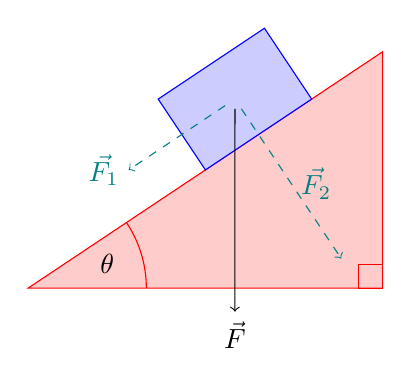
\begin{tikzpicture}[scale = 1.5]
\filldraw[draw = red, fill = red!20!white] (0,0) -- (3,2) -- (3,0) -- cycle;
\draw[red] (3,0) rectangle +(-0.2,0.2);
\draw[red] (1,0) arc [start angle = 0, end angle = 33.7, radius = 1];
\node at (16.8:0.7) {$\theta$};
\filldraw[draw = blue, fill = blue!20!white] (1.5,1) --++ (-0.4, 0.6) --++ (0.9, 0.6) --++ (0.4, -0.6) -- cycle;
\node at (1.75, 1.6) (A) {};
\draw[dashed, teal, ->] (A) --+ (-0.9, -0.6) node [left] {$\vec{F_1}$};
\draw[dashed, teal, ->] (A) --+ (0.9, -1.35) node [pos=0.5, right] {$\vec{F_2}$};
\draw[->] (A) -- (1.75, -0.2) node [below] {$\vec{F}$};
\end{tikzpicture}
\caption{การแปลงเวกเตอร์ $\vec{F}$ ออกเป็นเวกเตอร์ที่ขนานกับทิศทางการเคลื่อนที่}
\label{fig:vec_ortho_intro}
\end{figure}
\end{frame}

\begin{frame}
\frametitle{การฉายเชิงตั้งฉาก (orthogonal projection)}
\begin{defn}{}{}
กำหนดเวกเตอร์ $\vec{u}$ และ $\vec{b}$ แล้วเราสามารถเขียน
\begin{equation}
\vec{u} = \vec{w}_1 + \vec{w}_2
\end{equation}
โดยที่ $\vec{w}_1$ เรียกว่า \alert{ส่วนประกอบของเวกเตอร์ของ $\vec{u}$ ตาม $\vec{b}$} (หรือ โพรเจกชันตั้งฉากของ $\vec{u}$ บน $\vec{b}$) เขียนแทนด้วย $\vec{w}_1 = \text{Proj}_{\vec{b}} \vec{u}$ และ $\vec{w}_2$ เรียกว่า \alert{ส่วนประกอบเวกเตอร์ของ $\vec{u}$ ที่ตั้งฉากต่อ $\vec{b}$} 
\end{defn}
\end{frame}

\begin{frame}
\begin{figure}[h!]
\centering
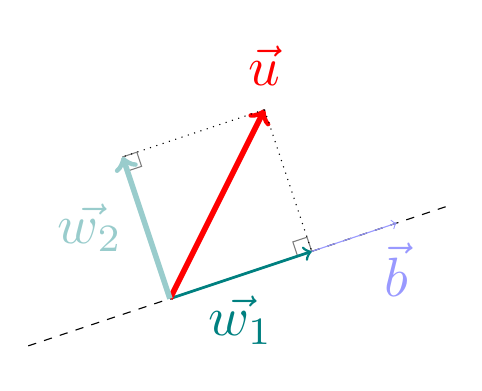
\begin{tikzpicture}[scale = 1.2, every node/.style={scale = 2}]
\draw[dashed] (-1.5,-0.5) -- (3,1);
\coordinate (b) at (2.4, 0.8);
\coordinate (u) at (1, 2);
\coordinate (w1) at (1.5, 0.5);
\coordinate (w2) at (-0.5, 1.5);
\draw[gray] (w1) --++ (-0.15,-0.05) --++ (-0.05, 0.15) --++ (0.15,0.05) -- cycle;
\draw[gray] (w2) --++ (0.15,0.05) --++ (0.05, -0.15) --++ (-0.15,-0.05) -- cycle;
\draw[->, blue!40!white] (0,0) -- (b) node[below] {$\vec{b}$};
\draw[->, teal, line width = 1pt] (0,0) -- (w1) node[below, pos=0.5] {$\vec{w_1}$};
\draw[->, red, line width = 2pt] (0,0) -- (u) node[above] {$\vec{u}$};
\draw[->, teal!40!white, line width = 2pt] (0,0) -- (w2) node[left, pos=0.5] {$\vec{w_2}$};
\draw[dotted] (u) -- (w1);
\draw[dotted] (u) -- (w2);
\end{tikzpicture}
\caption{ภาพแสดงส่วนประกอบของเวกเตอร์ของ $\vec{u}$ ตาม $\vec{b}$ และส่วนประกอบของเวกเตอร์ $\vec{u}$ ที่ตั้งฉากต่อ $\vec{b}$}
\label{fig:vec_ortho_intro}
\end{figure}

สามารถศึกษาเพิ่มเติมได้ที่\href{https://www.desmos.com/calculator/jlxdfi7law}{ลิงก์ desmos นี้}
\end{frame}

\begin{frame}[t]
\frametitle{วิธีการหาสูตร}
กำหนดเวกเตอร์ $\vec{u}$ และเวกเตอร์ $\vec{b}$ โดยที่ $\vec{b}$ แทนทิศทาง สมมติว่ามุมระหว่าง $\vec{u}$ และ $\vec{b}$ เป็นมุมแหลม (นั่นคือ $0 \leq \theta \leq \frac{\pi}{2})$

ถ้า $\vec{w_1}$ เป็นส่วนประกอบเวกเตอร์ของ $\vec{u}$ ตาม $\vec{b}$ แล้ว $\vec{w_1}$ จะมีสมบัติต่อไปนี้
\begin{slide}
\begin{tasks}[label = \arabic*)](1)
\task มีขนาดเท่ากับ $ \| \vec{u}\| \cos \theta$
\task มีทิศทางเดียวกันกับเวกเตอร์หนึ่งหน่วยในทิศทางของ $\vec{b}$ ซึ่งก็คือ $\frac{\vec{b}}{\| \vec{b}\|}$
\end{tasks}
\end{slide}
\end{frame}


\begin{frame}[t]
ฉะนั้น เราสามารถหา $\vec{w_1}$ ได้ดังนี้
\begin{slide}
\begin{eq*}
\vec{w_1} &=& \| \vec{u}\| \cos \theta \left( \frac{\vec{b}}{\| \vec{b}\|} \right) \\
&=& \frac{\vec{u} \cdot \vec{b}}{\| \vec{u}\| \|\vec{b} \|} \| \vec{u} \| \left( \frac{\vec{b}}{\| \vec{b}\|}\right) \\
&=& \frac{\vec{u} \cdot \vec{b}}{ \|\vec{b} \|^2} \vec{b}
\end{eq*}
\end{slide}
\end{frame}

\begin{frame}[t]
ในกรณีที่มุมระหว่าง $\vec{u}$ และ $\vec{b}$ เป็นมุมป้าน (นั่นคือ $\frac{\pi}{2} \leq \theta \leq \pi $) ให้เราใช้เวกเตอร์ $-\vec{b}$ แทน แต่อย่างไรก็ตาม สูตรที่ได้ออกมาเป็นสูตรดังนี้
\begin{slide}
\begin{eq*}
\vec{w_1} &=& \frac{\vec{u} \cdot (-\vec{b})}{ \|(-\vec{b}) \|^2} (-\vec{b}) \\
&=& \frac{(-1) (\vec{u} \cdot \vec{b}}{ ((-1)\|\vec{b} \|)^2} (-1)(\vec{b}) \\
&=& \frac{\vec{u} \cdot \vec{b}}{ \|\vec{b} \|^2} \vec{b} \\
\end{eq*}
ซึ่งสังเกตว่าเป็นสูตรเดียวกันกับสูตรแรก
\end{slide}
\end{frame}


\begin{frame}
\frametitle{การคำนวณการฉายเชิงตั้งฉาก}
\begin{thm}{}{}
กำหนดเวกเตอร์ $\vec{u}$ และ $\vec{b}$ ซึ่ง $\vec{b} \neq \vec{0}$ ถ้าเขียน $\vec{u} = \vec{w}_1 + \vec{w}_2$ ตามนิยามด้านบน แล้ว
\begin{eq} 
\vec{w}_1 &=& \text{Proj}_{\vec{b}} \vec{u} = \frac{\vec{u} \cdot \vec{b}}{\| \vec{b} \|^2} \vec{b} \label{eq:proj_formula_1} \\
\vec{w}_2 &=& \vec{u} - \vec{w}_1 \label{eq:proj_formula_2}
\end{eq}
\end{thm}
\end{frame}

\begin{frame}[t]
\begin{ex}
กำหนดให้ $\vec{u} = \bv{6, 3}$ และ $\vec{b} = \bv{3,4}$ จงหาส่วนประกอบเวกเตอร์ของ $\vec{u}$ ตาม $\vec{b}$ และส่วนประกอบเวกเตอร์ของ $\vec{u}$ ที่ตั้งฉากต่อ $\vec{b}$
\end{ex}
\begin{sol}
เราใช้สูตร \eqref{eq:proj_formula_1} ได้โดยคำนวณค่าต่อไปนี้ \pa
\begin{eq*}
\vec{u} \cdot \vec{b} \pa &=& \bv{6,3} \cdot \bv{3,4} \pa = (6)(3) + (3)(4) = 30 \pa \\
\| \vec{b} \|^2 \pa &=& (\sqrt{3^2 + 4^2})^2 \pa = 3^2 + 4^2 = 25
\end{eq*} \pa
ฉะนั้นส่วนประกอบเวกเตอร์ของ $\vec{u}$ ตาม $\vec{b}$ \pa คือ
\[\vec{w}_1 \pa = \text{Proj}_{\vec{b}}\vec{u} \pa \pa =  \frac{\vec{u} \cdot \vec{b}}{\| \vec{b} \|^2} \vec{b} \pa = \frac{30}{25} \bv{3,4} \pa = \bv{\frac{18}{5}, \frac{24}{5}}\pa = \bv{3.6, 4.8}\] \pa
และส่วนประกอบเวกเตอร์ของ $\vec{u}$ ที่ตั้งฉากต่อ $\vec{b}$ จาก \eqref{eq:proj_formula_2} \pa คือ
\[ \vec{w}_2 \pa = \vec{u} - \vec{w}_1 \pa = \bv{6,3} - \bv{3.6, 4.8} = \bv{2.4, -1.8}\]
\end{sol}
\end{frame}

\begin{frame}
\begin{figure}[h!]
\centering
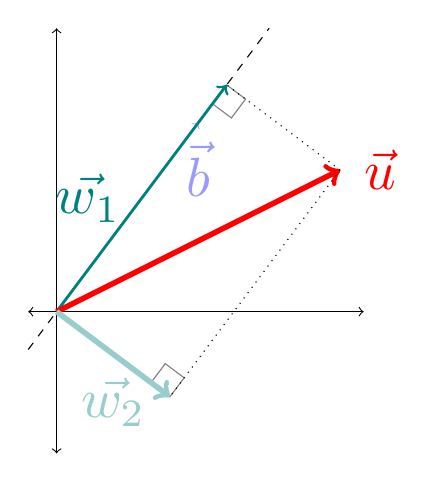
\begin{tikzpicture}[scale = 0.6, every node/.style={scale = 2}]
\draw[<->](-0.6,0)--(6.5,0);
\draw[<->](0,-3)--(0,6);
\draw[dashed] (-0.6,-0.8) -- (4.5,6);
\coordinate (b) at (3, 4);
\coordinate (u) at (6, 3);
\coordinate (w1) at (3.6, 4.8);
\coordinate (w2) at (2.4, -1.8);
\draw[gray] (w1) --++ (0.4,-0.3) --++ (-0.3, -0.4) --++ (-0.4, 0.3) -- cycle;
\draw[gray] (w2) --++ (0.3,0.4) --++ (-0.4, 0.3) --++ (-0.3,-0.4) -- cycle;
\draw[->, blue!40!white] (0,0) -- (b) node[below] {$\vec{b}$};
\draw[->, teal, line width = 1pt] (0,0) -- (w1) node[left, pos=0.5] {$\vec{w_1}$};
\draw[->, red, line width = 2pt] (0,0) -- (u) node[right] {$\vec{u}$};
\draw[->, teal!40!white, line width = 2pt] (0,0) -- (w2) node[below, pos=0.5] {$\vec{w_2}$};
\draw[dotted] (u) -- (w1);
\draw[dotted] (u) -- (w2);
\end{tikzpicture}
\caption{ภาพแสดงเวกเตอร์จากตัวอย่างที่ \theexample}
\label{fig:vec_ortho_ex1}
\end{figure}
\end{frame}

%%%%%%%%%%%%%
\section[ผลคูณไขว้]{ผลคูณไขว้ \\ (cross product)}
\frame{\sectionpage}
%%%%%%%%%%%%%

\begin{frame}
\frametitle{ที่มาของผลคูณไขว้}
เราได้ศึกษามาแล้วว่าการคูณจุดให้ผลลัพธ์เป็นปริมาณสเกลาร์ และมีค่าที่เกี่ยวข้องกับมุมระหว่างเวกเตอร์ ในที่นี้เราจะศึกษาการคูณอีกรูปแบบหนึ่งที่ให้ผลลัพธ์เป็นเวกเตอร์ โดยมีที่มาจากคำถามต่อไปนี้

\begin{question}
กำหนดเวกเตอร์ในปริภูมิสามมิติ $\vec{u}$ และ $\vec{v}$ แล้วจงหาเวกเตอร์ $\vec{w}$ ที่ตั้งฉากกับเวกเตอร์ทั้งสองนี้พร้อมกัน
\end{question}
\end{frame}

\begin{frame}
\begin{figure}[h!]
\centering
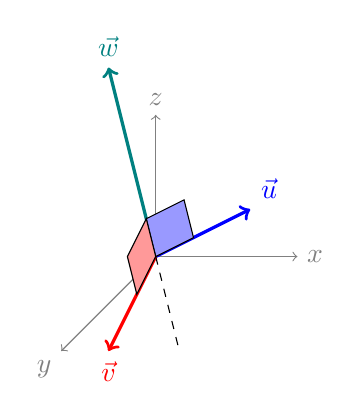
\begin{tikzpicture}[scale = 1.2]
\draw[->, gray] (0,0) -- (1.5,0) node[right] {$x$};
\draw[->, gray] (0,0) -- (-1,-1) node[below left] {$y$};
\draw[->, gray] (0,0) -- (0,1.5) node[above] {$z$};
\draw[->, very thick, blue] (0,0) -- (1,0.5) node [above right] {$\vec{u}$};
\draw[->, very thick, red] (0,0) -- (-0.5,-1) node [below] {$\vec{v}$};
\draw[->, very thick, teal] (0,0) -- (-0.5,2) node [above] {$\vec{w}$};
\draw[dashed] (0,0) -- (0.25,-1);
\filldraw[fill = blue!40!white] (0,0) --++ (-0.1,0.4) --++ (0.4, 0.2) --++ (0.1, -0.4) -- cycle;
\filldraw[fill = red!40!white] (0,0) --++ (-0.1,0.4) --++ (-0.2, -0.4) --++ (0.1, -0.4) -- cycle;
\end{tikzpicture}
\caption{ภาพแสดงเวกเตอร์ $\vec{w}$ ที่ตั้งฉากกับเวกเตอร์ $\vec{u}$ และ $\vec{v}$ พร้อมกัน}
\label{fig:vec_cross_prod_intro}
\end{figure}
\end{frame}

\begin{frame}
\frametitle{นิยามผลคูณไขว้}
\begin{slide}
\begin{defn}{}{}
กำหนดเวกเตอร์ $\vec{u} = \bv{u_1, u_2, u_3} $ และ $\vec{v} = \bv{v_1, v_2, v_3}$ ในปริภูมิ 3 มิติ แล้วผลคูณไขว้ (cross product) หรือผลคูณภายนอก (outer product) เขียนแทนด้วย $\vec{u} \times \vec{v}$ ซึ่งคำนวณได้จาก
\begin{eq}
&& \vec{u} \times \vec{v} = \left| \begin{array}{ccc} \vec{i} & \vec{j} & \vec{k} \\ u_1 & u_2 & u_3 \\ v_1 & v_2 & v_3 \end{array} \right| \label{eq:cross_formula_1} \\
&=& \vvv{(u_2v_3 - u_3v_2)}{+(u_3v_1 - u_1v_3)}{+(u_1v_2 - u_2v_1)} \label{eq:cross_formula_2}
\end{eq}
\end{defn}
\end{slide}
\end{frame}


\begin{frame}
\frametitle{วิธีช่วยจำผลคูณไขว้}
\begin{figure}[h!]
\centering
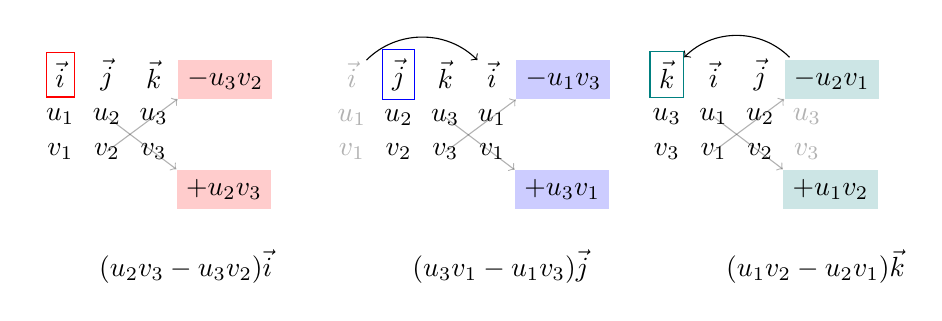
\begin{tikzpicture}
\matrix [ampersand replacement=\&]
{
	\node[draw = red] {$\vec{i}$};\& \node {$\vec{j}$};\&	 \node {$\vec{k}$}; \\
	\node {$u_1$};\&	 \node (1) {$u_2$};\&		 \node (2) {$u_3$}; \\
	\node {$v_1$};\&	 \node (3) {$v_2$};\&		\node (4){$v_3$}; \\
};
\draw[->, opacity = 0.3] (1.center) -- (4.south east) node [below right, opacity = 1, fill = red!20!white] {$+u_2 v_3$};
\draw[->, opacity = 0.3] (3.center) -- (2.north east) node [above right, opacity = 1, fill = red!20!white] {$-u_3 v_2$};
\node at (1,-2) {$(u_2v_3 - u_3v_2) \vec{i}$};
\begin{scope}[xshift = 4cm]
\matrix [column 1/.style ={nodes = {opacity = 0.3}}, ampersand replacement=\&]
{
	\node (A) {$\vec{i}$};\& \node[draw = blue] {$\vec{j}$};\&	 \node {$\vec{k}$}; \& \node (B) {$\vec{i}$};\\
	\node {$u_1$};\&	 \node {$u_2$};\&		 \node (1) {$u_3$}; \& \node (2) {$u_1$};\\
	\node {$v_1$};\&	 \node {$v_2$};\&		\node (3){$v_3$}; \& \node (4) {$v_1$};\\
};
\draw[->] (A) to [bend left=45] (B);
\draw[->, opacity = 0.3] (1.center) -- (4.south east) node [below right, opacity = 1, fill = blue!20!white] {$+u_3 v_1$};
\draw[->, opacity = 0.3] (3.center) -- (2.north east) node [above right, opacity = 1, fill = blue!20!white] {$-u_1 v_3$};
\node at (1,-2) {$(u_3v_1 - u_1v_3) \vec{j}$};
\end{scope}

\begin{scope}[xshift = 8cm]
\matrix [ampersand replacement=\&, column 4/.style={nodes={opacity = 0.3}}]
{
	\node[draw = teal] (A) {$\vec{k}$};  \& \node {$\vec{i}$};\& \node {$\vec{j}$};\&	 \node (B){$\vec{k}$}; \\
	\node {$u_3$}; \&	\node (1) {$u_1$};\&	 \node (2) {$u_2$};\&		 \node {$u_3$}; \\
	\node {$v_3$}; \&	\node (3) {$v_1$};\&	 \node (4) {$v_2$};\&		\node {$v_3$}; \\
};
\draw[->] (B) to [bend right=45] (A);
\draw[->, opacity = 0.3] (1.center) -- (4.south east) node [below right, opacity = 1, fill = teal!20!white] {$+u_1 v_2$};
\draw[->, opacity = 0.3] (3.center) -- (2.north east) node [above right, opacity = 1, fill = teal!20!white] {$-u_2 v_1$};
\node at (1,-2) {$(u_1v_2 - u_2v_1) \vec{k}$};
\end{scope}
\end{tikzpicture}
\caption{วิธีช่วยจำผลคูณไขว้}
\end{figure}
\end{frame}


\begin{frame}[t]
\begin{ex}
กำหนดให้ $\vec{u} = \bv{0,1,2}$ และ $\vec{v} = \bv{3,4,5}$ จงหา $\vec{u} \times \vec{v}$
\end{ex}
\begin{sol}
ใช้สูตร \eqref{eq:cross_formula_2} จะได้ \pa
\begin{eq*}
\vec{u} \times \vec{v} \pa \pa &=&  \vvv{(u_2v_3 - u_3v_2)}{+(u_3v_1 - u_1v_3)}{+(u_1v_2 - u_2v_1)} \pa \\
\pa &=& \vvv{((1)(5) - (4)(2))}{+((2)(3) - (0)(5))}{ + ((0)(4) - (1)(3))} \pa \\
\pa &=& \vvv{(5-8)}{+(6-0)}{+(0-3)}\pa \\
\pa &=& \vvv{-3}{+6}{-3} \pa \\
\pa &=& \bv{-3, 6, -3}
\end{eq*}
\end{sol}
\end{frame}

\begin{frame}
\frametitle{ผลคูณไขว้ของเวกเตอร์ในปริภูมิ 2 มิติ}
\begin{slide}
ถ้า $\vec{u} = \bv{u_1, u_2} $ และ $\vec{v} = \bv{v_1, v_2}$ เป็นเวกเตอร์ในปริภูมิ 2 มิติ ในบางครั้งเราสามารถใช้ผลคูณไขว้เพื่อคำนวณค่าบางค่าได้อย่างสะดวกขึ้น ในกรณีนี้เราจะมองว่า $\vec{u}$ และ $\vec{v}$ เป็นเวกเตอร์ในปริภูมิ 3 มิติ โดยเขียนใหม่เป็น
\begin{eq*}
\vec{u} &=& \vv{u_1}{+u_2} = \vvv{u_1}{+u_2}{+0} = \bv{u_1, u_2, 0} \\
\vec{v} &=& \vv{v_1}{+v_2} = \vvv{v_1}{+v_2}{+0} = \bv{v_1, v_2, 0}
\end{eq*}
ฉะนั้น
\begin{block}{}
\[ \vec{u} \times \vec{v} = \left| \begin{array}{ccc} \vec{i} & \vec{j} & \vec{k} \\ u_1 & u_2 & 0 \\ v_1 & v_2 & 0 \end{array} \right| = (u_1v_2 - u_2v_1)\bvec{k} \]
\end{block}
สังเกตว่าผลลัพธ์เป็นเวกเตอร์ที่ขนานกับเวกเตอร์ $\bvec{k}$ นั่นคือขนานกับแกน $z$
\end{slide}
\end{frame}

\begin{frame}
\frametitle{สมบัติของผลคูณไขว้}
\begin{prop}{}{}
กำหนดเวกเตอร์ $\vec{u}, \vec{v}$ และ $\vec{w}$ ในปริภูมิสามมิติ และค่าคงตัว $k$
\begin{enumerate}
\item $\vec{u} \times \vec{v} = - (\vec{v} \times \vec{u})$
\item $\vec{u} \times (\vec{v}+ \vec{w}) = \vec{u} \times \vec{v} + \vec{u} \times \vec{w}$
\item $k (\vec{u} \times \vec{v}) = (k \vec{u}) \times \vec{v} = \vec{u} \times (k\vec{v})$
\item $\vec{u} \times \vec{u} = \vec{0}$
\item $\vec{u} \times \vec{0} = \vec{0} \times \vec{u} = \vec{0}$
\end{enumerate}
\end{prop}
\end{frame}

\begin{frame}
\frametitle{พื้นที่ของสี่เหลี่ยมด้านขนาน}
\begin{thm}{}{}
กำหนดให้ $\theta$ เป็นมุมระหว่างเวกเตอร์ $\vec{u}$ และ $\vec{v}$ และให้ $A$ เป็นพื้นที่ของสี่เหลี่ยมด้านขนานที่เกิดจากเวกเตอร์ $\vec{u}$ และ $\vec{v}$ แล้ว
\begin{eq}
A &=& \| \vec{u} \| \|\vec{v}\| \sin \theta\\
&=& \| \vec{u} \times \vec{v} \| 
\end{eq}
\end{thm}
ข้อสังเกต: เราสามารถใช้ผลคูณไขว้ในการหามุม $\theta$ ระหว่างเวกเตอร์ ได้ดังนี้
\[\sin \theta = \frac{ \| \vec{u} \times \vec{v} \| }{\| \vec{u} \| \|\vec{v}\| }\]
\end{frame}

\begin{frame}
\begin{figure}[h!]
\centering
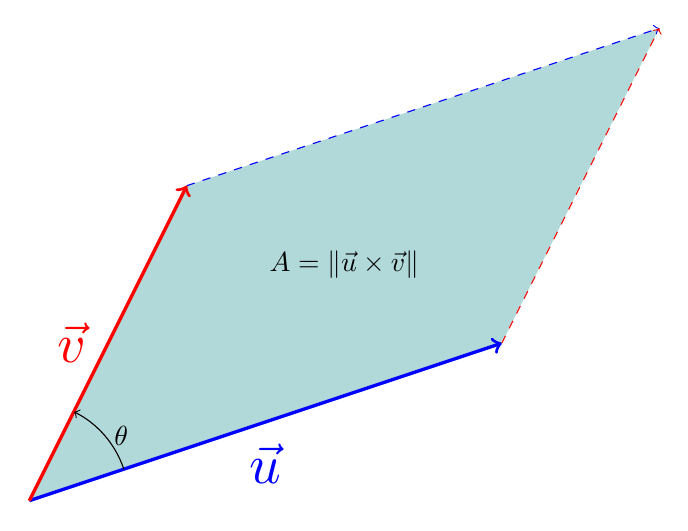
\begin{tikzpicture}[scale = 2]
\fill[fill = teal!30!white] (0,0) -- (3,1) -- (4,3) -- (1,2) -- cycle;
\draw[->, blue, very thick] (0,0) -- (3,1) node [below, pos = 0.5, scale = 2] {$\vec{u}$};
\draw[->, blue, dashed] (1,2) -- (4,3);
\draw[->, red, very thick] (0,0) -- (1,2) node [left, pos = 0.5, scale = 2] {$\vec{v}$};
\draw[->, red, dashed] (3,1) -- (4,3);
\draw[->] (0.6,0.2) arc [start angle = 18.43, end angle = 63.43, radius = 0.63] node [pos=0.5, right] {$\theta$};
\node at (2,1.5) {$A = \| \vec{u} \times \vec{v} \|$};
\end{tikzpicture}
\caption{พื้นที่ของสี่เหลี่ยมด้านขนานที่เกิดจากเวกเตอร์ $\vec{u}$ และ $\vec{v}$}
\end{figure}
\end{frame}

\begin{frame}[t]
\begin{ex}
จงหาพื้นที่ของสี่เหลี่ยมด้านขนานที่เกิดจากเวกเตอร์ $\bv{1,2,3}$ และเวกเตอร์ $\bv{0,4,5}$
\end{ex}
\begin{sol}
เราใช้สูตร \ref{eq:vector_cross_prod_area} ได้ทันทีดังนี้

\begin{eq*}
&&\bv{1,2,3} \times \bv{0,4,5} \\
&=& \vvv{((2)(5) - (3)(4))}{+((3)(0) - (1)(5))}{+((1)(4)-(0)(2))} \\
&=& \vvv{-2}{-5}{+4}
\end{eq*}
ฉะนั้นพื้นที่ของสี่เหลี่ยมด้านขนานมีค่าเท่ากับ
\begin{eq*}
A = \| \vvv{-2}{-5}{+4} \| &=& \sqrt{(-2)^2 + (-5)^2 + (4)^2} \\
&=& \sqrt{4+25+16} = \sqrt{45} = 3\sqrt{5}
\end{eq*}
\end{sol}
\end{frame}


\begin{frame}
\frametitle{ผลคูณเชิงสเกลาร์ของสามเวกเตอร์}
\begin{slide}
ข้อควรระวังของการคูณเวกเตอร์คือ เราไม่สามารถรวมผลคูณจุดและผลคูณไขว้กันได้เสมอไป เช่น
\[\red{ (\vec{u} \cdot \vec{v}) \cdot \vec{w}} \]
นั้น\textbf{ไม่}สามารถทำได้ เนื่องจาก $\vec{u} \cdot \vec{v}$ เป็นจำนวนจริง ซึ่งเราไม่สามารถหาผลคูณจุดระหว่างจำนวนจริง $(\vec{u} \cdot \vec{v})$ กับเวกเตอร์ $\vec{w}$ ได้ แต่เราสามารถหาผลคูณ
\[ (\vec{u} \cdot \vec{v}) \vec{w} \]
ได้ โดยตัวอย่างผลคูณแบบอื่น ได้แก่
\[ (\vec{u} \cdot \vec{v}) \vec{w}, \quad \vec{u} \cdot (\vec{v} \times \vec{w}), \quad \vec{u} \times (\vec{v} \times \vec{w}) \]
ซึ่งผลคูณแต่ละตัวนั้นมีความหมายแตกต่างกันไป
\end{slide}
\end{frame}

\begin{frame}
\frametitle{ความหมายของผลคูณเชิงสเกลาร์ของสามเวกเตอร์}
\begin{thm}{}{}
กำหนดเวกเตอร์ $\vec{u} = \bv{u_1, u_2, u_3}, \vec{v} = \bv{v_1, v_2, v_3}$ และ $ \vec{w} = \bv{w_1, w_2, w_3}$ ในปริภูมิ 3 มิติ แล้ว
\begin{equation}
\vec{u} \cdot (\vec{v} \times \vec{w}) = u_1(v_2w_3 - v_3w_2) +u_2(v_3w_1 - v_1w_3)+u_3(v_1w_2 - v_2w_1) \label{eq:triple_product}
\end{equation}
ถ้าให้ $V$ เป็นปริมาตรของทรงสี่เหลี่ยมด้านขนานที่มี $\vec{u}, \vec{v}$ และ $\vec{w}$ เป็นขอบแล้ว
\[ V = | \vec{u} \cdot (\vec{v} \times \vec{w}) |\]
\end{thm}
\end{frame}

\begin{frame}
\begin{figure}[h!]
\centering
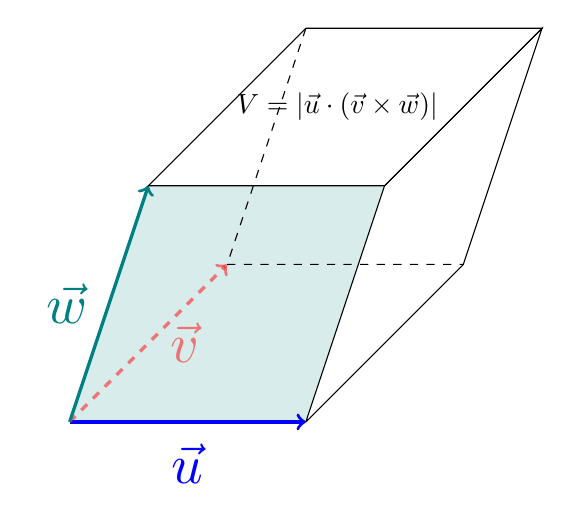
\begin{tikzpicture}
\fill[teal!30!white, opacity = 0.5] (0,0) -- (3,0) -- (4,3) -- (1,3) -- cycle;
\draw[->, blue, very thick] (0,0) -- (3,0) node [below, pos = 0.5, scale = 2] {$\vec{u}$};
\draw[->, red, very thick, dashed, opacity = 0.5] (0,0) -- (2,2) node [right, pos = 0.5, scale = 2] {$\vec{v}$};
\draw[->, teal, very thick] (0,0) -- (1,3) node [left, pos = 0.5, scale = 2] {$\vec{w}$};
\draw (1,3) --++ (2,2) --++ (3,0) --++ (-2,-2) -- cycle;
\draw[dashed] (3,5) --++ (-1,-3) --++ (3,0);
\draw (3,0) --++ (1,3) --++ (2,2) --++ (-1,-3) --++ (-2,-2);
\node at (3.4,4) {$V = |\vec{u} \cdot ( \vec{v} \times \vec{w} )|$};
\end{tikzpicture}
\caption{ปริมาตรของทรงสี่เหลี่ยมด้านขนานที่เกิดจากเวกเตอร์ $\vec{u}$, $\vec{v}$ และ $\vec{w}$}
\end{figure}
\end{frame}

 
\begin{frame}[t] 
\begin{ex}
กำหนดเวกเตอร์ $\vec{u} = \bv{2,-3,0}, \vec{v} = \bv{1,1,-1}$ และ $\vec{w} = \bv{3,0,-1}$ จงหาปริมาตรของทรงสี่เหลี่ยมด้านขนาน ที่มี $\vec{u}, \vec{v}$ และ $\vec{w}$ เป็นขอบ
\end{ex} 
\begin{sol}
ใช้สูตร \eqref{eq:triple_product} ทันที จะได้ 
\begin{eq*}
&&\vec{u} \cdot (\vec{v} \times \vec{w}) \\
&=& (2)((1)(-1) - (-1)(0)) \\
&& +(-3)((-1)(3) - (1)(-1)) \\
&& +(0)((1)(0) - (1)(3)) \\
&=& (2)(-1) + (-3)(-2) = 4
\end{eq*}
นั่นคือ ทรงสี่เหลี่ยมด้านขนานมีปริมาตร 4 ลูกบาศก์หน่วย
\end{sol}
\end{frame}

